%%%%%%%%%%%%%%%%%%%%%%%%%%%%%%%%%%%%%%%%%
% Developer CV
% LaTeX Template
% Version 1.0 (28/1/19)
%
% This template originates from:
% http://www.LaTeXTemplates.com
%
% Authors:
% Jan Vorisek (jan@vorisek.me)
% Based on a template by Jan Küster (info@jankuester.com)
% Modified for LaTeX Templates by Vel (vel@LaTeXTemplates.com)
%
% License:
% The MIT License (see included LICENSE file)
%
%%%%%%%%%%%%%%%%%%%%%%%%%%%%%%%%%%%%%%%%%

%----------------------------------------------------------------------------------------
%	PACKAGES AND OTHER DOCUMENT CONFIGURATIONS
%----------------------------------------------------------------------------------------

\documentclass[9pt]{developercv} % Default font size, values from 8-12pt are recommended


%----------------------------------------------------------------------------------------
% Для успешной сборки требуется добавить хуки в .git или
% отключить данный usepackage для случая черновой сборки
% Официальные версии генерируются только с включенной опцией
% Особенности файла .git/gitHeadInfo.gin:
% - Нельзя автора с не латинским именем (поля authname, commname)
% - Нельзя названия веток в формате чисел (поле refnames)
% Иначе будут малопонятные ошибки сборки.
\RequirePackage[mark]{gitinfo2}
%----------------------------------------------------------------------------------------

\usepackage{csquotes}
\usepackage{paralist}

\newgeometry{top=1cm,bottom=1cm,right=1cm,left=1cm}

\begin{document}


	%! Author = Андрей
%! Date = 05.11.2022

%----------------------------------------------------------------------------------------
%	TITLE AND CONTACT INFORMATION
%----------------------------------------------------------------------------------------

	\begin{minipage}{0.1\textwidth}
		\begin{figure}[H]
			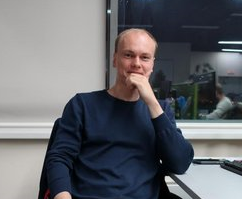
\includegraphics[width=3.5cm]{1}
		\end{figure}
	\end{minipage}
	\hfill
    \begin{minipage}[t]{0.35\textwidth} % 45% of the page width for name
        %\vspace{-\baselineskip} % Required for vertically aligning minipages

        % If your name is very short, use just one of the lines below
        % If your name is very long, reduce the font size or make the minipage wider and reduce the others proportionately
        \colorbox{black}{{\HUGE\textcolor{white}{\textbf{\MakeUppercase{Andrei}}}}} % First name

        \colorbox{black}{{\HUGE\textcolor{white}{\textbf{\MakeUppercase{Briukhov}}}}} % Last name

        \vspace{6pt}

        {\huge Java/Kotlin developer} % Career or current job title
    \end{minipage}
    \begin{minipage}[t]{0.25\textwidth} % 27.5% of the page width for the first row of icons
        %\vspace{-\baselineskip} % Required for vertically aligning minipages

        % The first parameter is the FontAwesome icon name, the second is the box size and the third is the text
        % Other icons can be found by referring to fontawesome.pdf (supplied with the template) and using the word after \fa in the command for the icon you want
        %\icon{MapMarker}{12}{}\\

        \icon{Globe}{12}{Brazil, São Paulo}\\
        \icon{Calendar}{12}{25-05-1986, 36 yo}\\
        \icon{Phone}{12}{+55 (11) 97791-8776}\\
        \icon{At}{12}{\href{mailto:andreybr611@gmail.com}{andreybr611@gmail.com}}

    \end{minipage}
    \begin{minipage}[t]{0.2\textwidth} % 27.5% of the page width for the second row of icons
        %\vspace{-\baselineskip} % Required for vertically aligning minipages

        % The first parameter is the FontAwesome icon name, the second is the box size and the third is the text
        % Other icons can be found by referring to fontawesome.pdf (supplied with the template) and using the word after \fa in the command for the icon you want
        \icon{Linkedin}{12}{\href{https://www.linkedin.com/in/tbw777}{tbw777}} \\
        \icon{Skype}{12}{\href{https://join.skype.com/invite/mjNUCTfkejKc}{Click to chat}} \\
        \icon{Twitter}{12}{\href{https://twitter.com/ABriukhov}{ABriukhov}} \\
        \icon{Whatsapp}{12}{\href{https://wa.me/5511977918776}{Click to chat}}\\
%        \icon{MessageText}{12}{Generated in \LaTeX}
    \end{minipage}



    \vspace{0.4cm}

%----------------------------------------------------------------------------------------
%	INTRODUCTION, SKILLS AND TECHNOLOGIES
%----------------------------------------------------------------------------------------

    \begin{minipage}[t]{0.76\textwidth} % 40% of the page width for the introduction text
        \vspace{-\baselineskip} % Required for vertically aligning minipages
        
        \cvsect{Why me?}

        \begin{itemize}[leftmargin=.0in]
        	\setlength\itemsep{0em}
            \item I understand the structure of systems, possible schemes for building interactions and frequent mistakes
            \item I develop safe and reliable systems with highest quality of code maintability and extensability
            \item I prefer versatility, consistency, always looking for systemic scalable automated solutions
            \item I adhere to the principles: \textbf{SDLC}, \textbf{SOLID}, \textbf{KISS}, \textbf{DRY}, \textbf{YAGNI}, and the typical architecture and design patterns
            \item I choose approaches and prioritize based on context and requirements
            \item My overall experience is about \underline{17} years of commercial development (since 2005)
            \item Successful experience in solving business-critical project tasks from the first job
        \end{itemize}

    \end{minipage}
    \hfill % Whitespace between
    \begin{minipage}[t]{0.20\textwidth} % 50% of the page for the skills bar chart
        \vspace{-\baselineskip}
        
        \cvsect{My stack}
        
        \icon{Java}{10}{\textbf{Java}} \& \textbf{Kotlin} plus:
        \begin{itemize}[leftmargin=.2in]
        	\setlength\itemsep{0em}
        	\item Assembler
        	\item Camunda
        	\item C/C++
           	\item Groovy
           	\item JavaScript
           	\item Shell script
            
            %\item{JavaScript: Node.js, JQuery, React, Angular}
            %\item{C/C++ (C89/C99/C++2003/Other)}
            %\item{Assembler x86: real mode, unreal mode, protected mode, MSRs}
            
            \item \LaTeX
        \end{itemize}
    \end{minipage}

\vspace{0.4cm}
	%! Author = Андрей
%! Date = 05.11.2022

%----------------------------------------------------------------------------------------
%	EXPERIENCE
%----------------------------------------------------------------------------------------

\cvsect{EXPERIENCE}

\begin{entrylist}
    \entry
    {09/2022\\\footnotesize{One-time request}}
    {Consultant}
    {\enquote{RSHB} bank}
    {
        Provided analysis and recommendations for project restructuring and task management
    }

    \entry
    {02/2021 -- 07/2022\\\footnotesize{1 year 6 months\\full time + weekends}}
    {Head}
    {Fazum at Moscow Innovation Center \enquote{Skolkovo}}
    {
        Built a NetBeans RCP (non-ide) based solution \\
    Created new Camunda processes and services with Spring (including Swagger/OpenAPI/Feign) and Gradle \\
    Created self-generated universal documentation with Git and LaTeX \\
    Created a reporting service that generate data for Power BI form different sources: Jira, Elastic, Kelycloak \\
    Provided daily bank queries on the platform \\
    \texttt{Java 6-17}\slashsep\texttt{SQL}\slashsep\texttt{Camunda}\slashsep\texttt{Kotlin}\slashsep\texttt{Elastic}\slashsep\texttt{Linux}\slashsep\texttt{Docker}\slashsep\texttt{Swagger \& OpenAPI}
    }

    \entry
    {05/2018 -- 02/2021\\\footnotesize{2 years 10 months\\full time}}
    {Team lead}
    {MOCIKT}
    {
        Maintenance and development of the service portal \url{https://uslugi.mosreg.ru} \\
        Transferred projects from a supplier \\
        Completed design and development of new services \\
        Fixed supplier errors in production \\
        Task training for colleagues was done \\
        Task/code review \\
        Interaction with other departments when coupling systems \\
        Help colleagues solve various problems \\
        Productivity monitoring, hot fixes \\
    Team size about 8 workers: (back and front developers, devops, other) \\
    \texttt{Java 4-15}\slashsep\texttt{Kotlin}\slashsep\texttt{Spring}\slashsep\texttt{Postgres}\slashsep\texttt{Elastic}\slashsep\texttt{Gitlab CI}\slashsep\texttt{Teamcity}\slashsep\texttt{Docker}
	}

    \entry
    {08/2017 -- 05/2018\\\footnotesize{10 months\\full time + weekends}}
    {Java Developer}
    {PSB Bank}
    {
        Support and development of Java EE applications \\
        \texttt{Java SE 8 \& Java EE 6}\slashsep\texttt{Oracle SQL}\slashsep\texttt{IBM WebSphere}
    }
    
    \entry
    {07/2017 -- 08/2017\\\footnotesize{2 months\\full time}}
    {Java Developer}
    {Paramitec}
    {
        Support and development of Ministry of Foreign Affairs apps. \\
        I did leave after get an offer from PS Bank. \\
        \texttt{Java 8}\slashsep\texttt{PostgreSQL}\slashsep\texttt{Tomcat}
    }
    
    \entry
    {01/2016 -- 06/2017\\\footnotesize{1 year 6 months\\full time}}
    {Java EE/Android/Node.js/PHP developer}
    {Octopod}
    {
        Created an extension in CUBA.platform \\
        Researched the thesis and docsvision workflow system for the possibility of expansion \\
        Developed a mini site using a graphical database \\
        Developed a mobile application for the company X5 \\
        Developed a chatbot for microsoft digital forum 2016 \\
        Developed corporate JAX-RS (Java EE) application for mobile devices\\
    \texttt{Java 8}\slashsep\texttt{Websphere}\slashsep\texttt{Hibernate}\slashsep\texttt{Cuba}\slashsep\texttt{Android}\slashsep\texttt{SAP OData}\slashsep\texttt{Node.js}\slashsep\texttt{bots}
	}
    
    \entry
    {04/2013 -- 09/2015\\\footnotesize{2 years 6 months\\full time}}
    {Java Developer}
    {Supertel}
    {
        Support and maintenance of a two versions telecommunications software system \\
        Provided analysis and recommendations for an old assembler project \\
        \texttt{Java 7}\slashsep\texttt{SNMP}\slashsep\texttt{Maven}\slashsep\texttt{JUnit}\slashsep\texttt{PostreSQL}\slashsep\texttt{Glassfish}\slashsep\texttt{NetBeans RCP}
    }

    \entry
    {07/2005 -- 03/2013\\\footnotesize{7 years 9 months\\full time}}
    {Software Developer}
    {Radioavionika}
    {
        Developed many components for real-time operating system:
        \begin{itemize}[leftmargin=.2in]
        	\setlength\itemsep{0em}
            \item Intel x86 protected mode implementation
            \item Multilevel real-time security control subsystem
            \item Multilevel real-time execution self tests
            \item 16/32bit boot loaders with mem hacks and using unreal mode
            \item Own PE/DLL linker to provide ROM section support
            \item Flexible logs generators
            \item Varios programs for analysis logs, memory and compilation stages
            \item VESA drivers
            \item Thin automated client to intellectual load data on hardware without monitor
            \item Documentation for components
            \item Several experimental programs for KolibriOS: cache control and code timings measure
        \end{itemize}
    \texttt{FASM \& TASM}\slashsep\texttt{Bochs}\slashsep\texttt{Linux}\slashsep\texttt{GCC}\slashsep\texttt{Doxygen}\slashsep\texttt{C \& C++}\slashsep\texttt{Gimpel PC Lint}\slashsep\texttt{Java 6}}

\end{entrylist}


	%----------------------------------------------------------------------------------------
%	EDUCATION
%----------------------------------------------------------------------------------------

\cvsect{Education}

\begin{entrylist}
    \entry
    {2003 -- 2010}
    {Specialist}
    {Petersburg University of Information Technology, Mechanics and Optics}
    {Specialty: Information security organization and technology}
\end{entrylist}

	%! Author = Андрей
%! Date = 05.11.2022


\begin{minipage}[t]{0.76\textwidth}
    \vspace{-\baselineskip} % Required for vertically aligning minipages

    \cvsect{Publications}

    ISBN: 5–98052–111–9: Saint-Petersburg, \enquote{Radioavionica}.                                     \\
    \textit{\enquote{MULTIPURPOSE RADIO-ELECTRONIC COMPLEXES}: collection of scientific articles}.\\
    Anniversary Edition. Polytechnic University press, 2011. - 400 pages.                               \\
    The book PDF file (clickable): \url{http://www.radioavionica.ru/about/events/knigi-i-sborniki/312/}\\
    My articles:
    \begin{itemize}
        \setlength\itemsep{0em}
        \item \textit{Static and dynamic error detection systems in source and executable software code}. pp 189-192.
        \item \textit{Security benchmarking of real-time operating systems}. pp 193-195.
    \end{itemize}

\end{minipage}
\hfill
\begin{minipage}[t]{0.2\textwidth}
    \vspace{-\baselineskip} % Required for vertically aligning minipages

    \cvsect{Tests}
    \icon{Code}{12}{\href{https://leetcode.com/tbw777/}{LeetCode}}\\
%    \icon{Code}{12}{\href{https://www.codewars.com/users/tbw777}{CodeWars}}

    \cvsect{Code}
    \icon{Github}{12}{\href{https://github.com/tbw777}{tbw777}}
\end{minipage}

\vspace{0.4cm}
	%! Author = Андрей
%! Date = 05.11.2022

%----------------------------------------------------------------------------------------
%	ADDITIONAL INFORMATION
%----------------------------------------------------------------------------------------

\begin{minipage}[t]{0.3\textwidth}
    \vspace{-\baselineskip} % Required for vertically aligning minipages

    \cvsect{Línguas}

    \textbf{Russo} - main\\
    \textbf{Inglês} - B1\\
    %\textcolor{red}{\textbf{Spanish} - A1}\\
    \textcolor{red}{\textbf{Portuguese} - no processo de estudar}
\end{minipage}
\hfill
\begin{minipage}[t]{0.3\textwidth}
    \vspace{-\baselineskip} % Required for vertically aligning minipages

    \cvsect{Hobbies}

    \textbf{Esporte} \\
    \textbf{Motocicletas}

\end{minipage}
\hfill
\begin{minipage}[t]{0.3\textwidth}
    \vspace{-\baselineskip} % Required for vertically aligning minipages

    \cvsect{Outro}

    \textbf{No processo de escrever o livro \enquote{Aplicativos NetBeans Simples}}
\end{minipage}

%----------------------------------------------------------------------------------------

	%! Author = Андрей
%! Date = 06.11.2022

\cvsect{Computador}

\begin{entrylist}
    \entry
    {02/2021}
    {Computador portátil}
    {Ter um trabalho em todos os lugares e concluir com sucesso qualquer tipo de tarefa}
    {
        ASUSTeK COMPUTER INC. ROG Strix G733QS\_G733QS             \\
        RAM 64                                                     \\
        AMD Ryzen 9 5900HX with Radeon Graphics, 3301 MHz, 8 cores \\
    NVIDIA GeForce RTX 3080                                    \\
    Webcam 1280p\\

    Como mostra a experiência de trabalhar remotamente, você pode se concentrar significativamente melhor nas tarefas de trabalho e obter ótimos resultados.
    Mas para a organização você precisa ser capaz de escolher uma pessoa responsável
    }
\end{entrylist}

	\cvsect{FAQ}

\begin{entrylist}
    \entry
    {}
    {Em quanto tempo você poderia começar a trabalhar conosco?}
    {}
    {
        Eu preciso de uma semana.
    }
\end{entrylist}

	%\input{content/legal}

\end{document}
